\pagebreak
\subsection{Ground Support Equipment}\label{sec:4.9}
A \st{computer} \hl{laptop} on the ground will be connected to the experiment via the E-Link. \hl{A spare laptop will be kept close-by should any problems arise with the main one.} The ground support software will include a simple GUI which will enable an operator to issue commands to the experiment such as reset, target selection, and moving to landing position. Compressed pictures will be received by the ground support software, which can be examined to verify nominal operation. \hl{The ground support software will be written in C and Python, using GTK+ to build the GUI.} \st{The ground support software will be written in C.}

\begin{figure}[h]
	\centering
	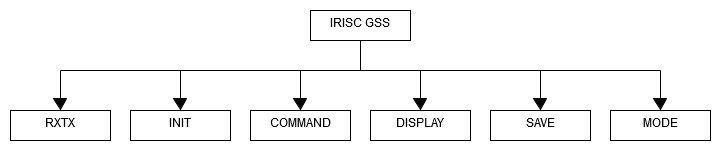
\includegraphics[width=\textwidth]{4-experiment-design/img/software/GSS-tree.png}
	\caption{Design tree of IRISC Ground Support Software}
	\label{fig:gss-tree}
\end{figure}

The ground support software that will be running is shown in figure \ref{fig:gss-tree}. The RXTX object will send and receive data via the E-link. The INIT object initializes the software. The COMMAND object reads and parses commands sent by the user through the GUI, which will also be used by the DISPLAY object to show received data to the user. The SAVE object is used to save the received data to local storage, and lastly the MODE object handles the modes of the software.
\raggedbottom
